%!TEX root = ../Studienarbeit.tex

In diesem Kapitel sollen die Beweggründe, sowie die geplante Vorgehensweise zur \titel erläutert werden.


\section{Motivation}

Der Anstieg der Waschbärenpopulation in vielen Teilen Deutschlands hat zu Schäden in Gärten, Parks und Friedhöfen geführt. Auch der eigene Garten ist davon leider nicht unversehrt geblieben, was in Abbildung \ref{fig:Garten} zu sehen ist. Die üblichen Mittel wie Ultraschall- und Blitzlicht- Abschrecksystemen scheinen nur von sehr kurzer Dauer einen Erfolg zu bieten. Angesichts dessen ist die Entwicklung eines effektiven Abwehrsystems gegen Waschbären von entscheidender Bedeutung, um weitere Schäden zu minimieren.


\begin{figure}[h]
    \centering
    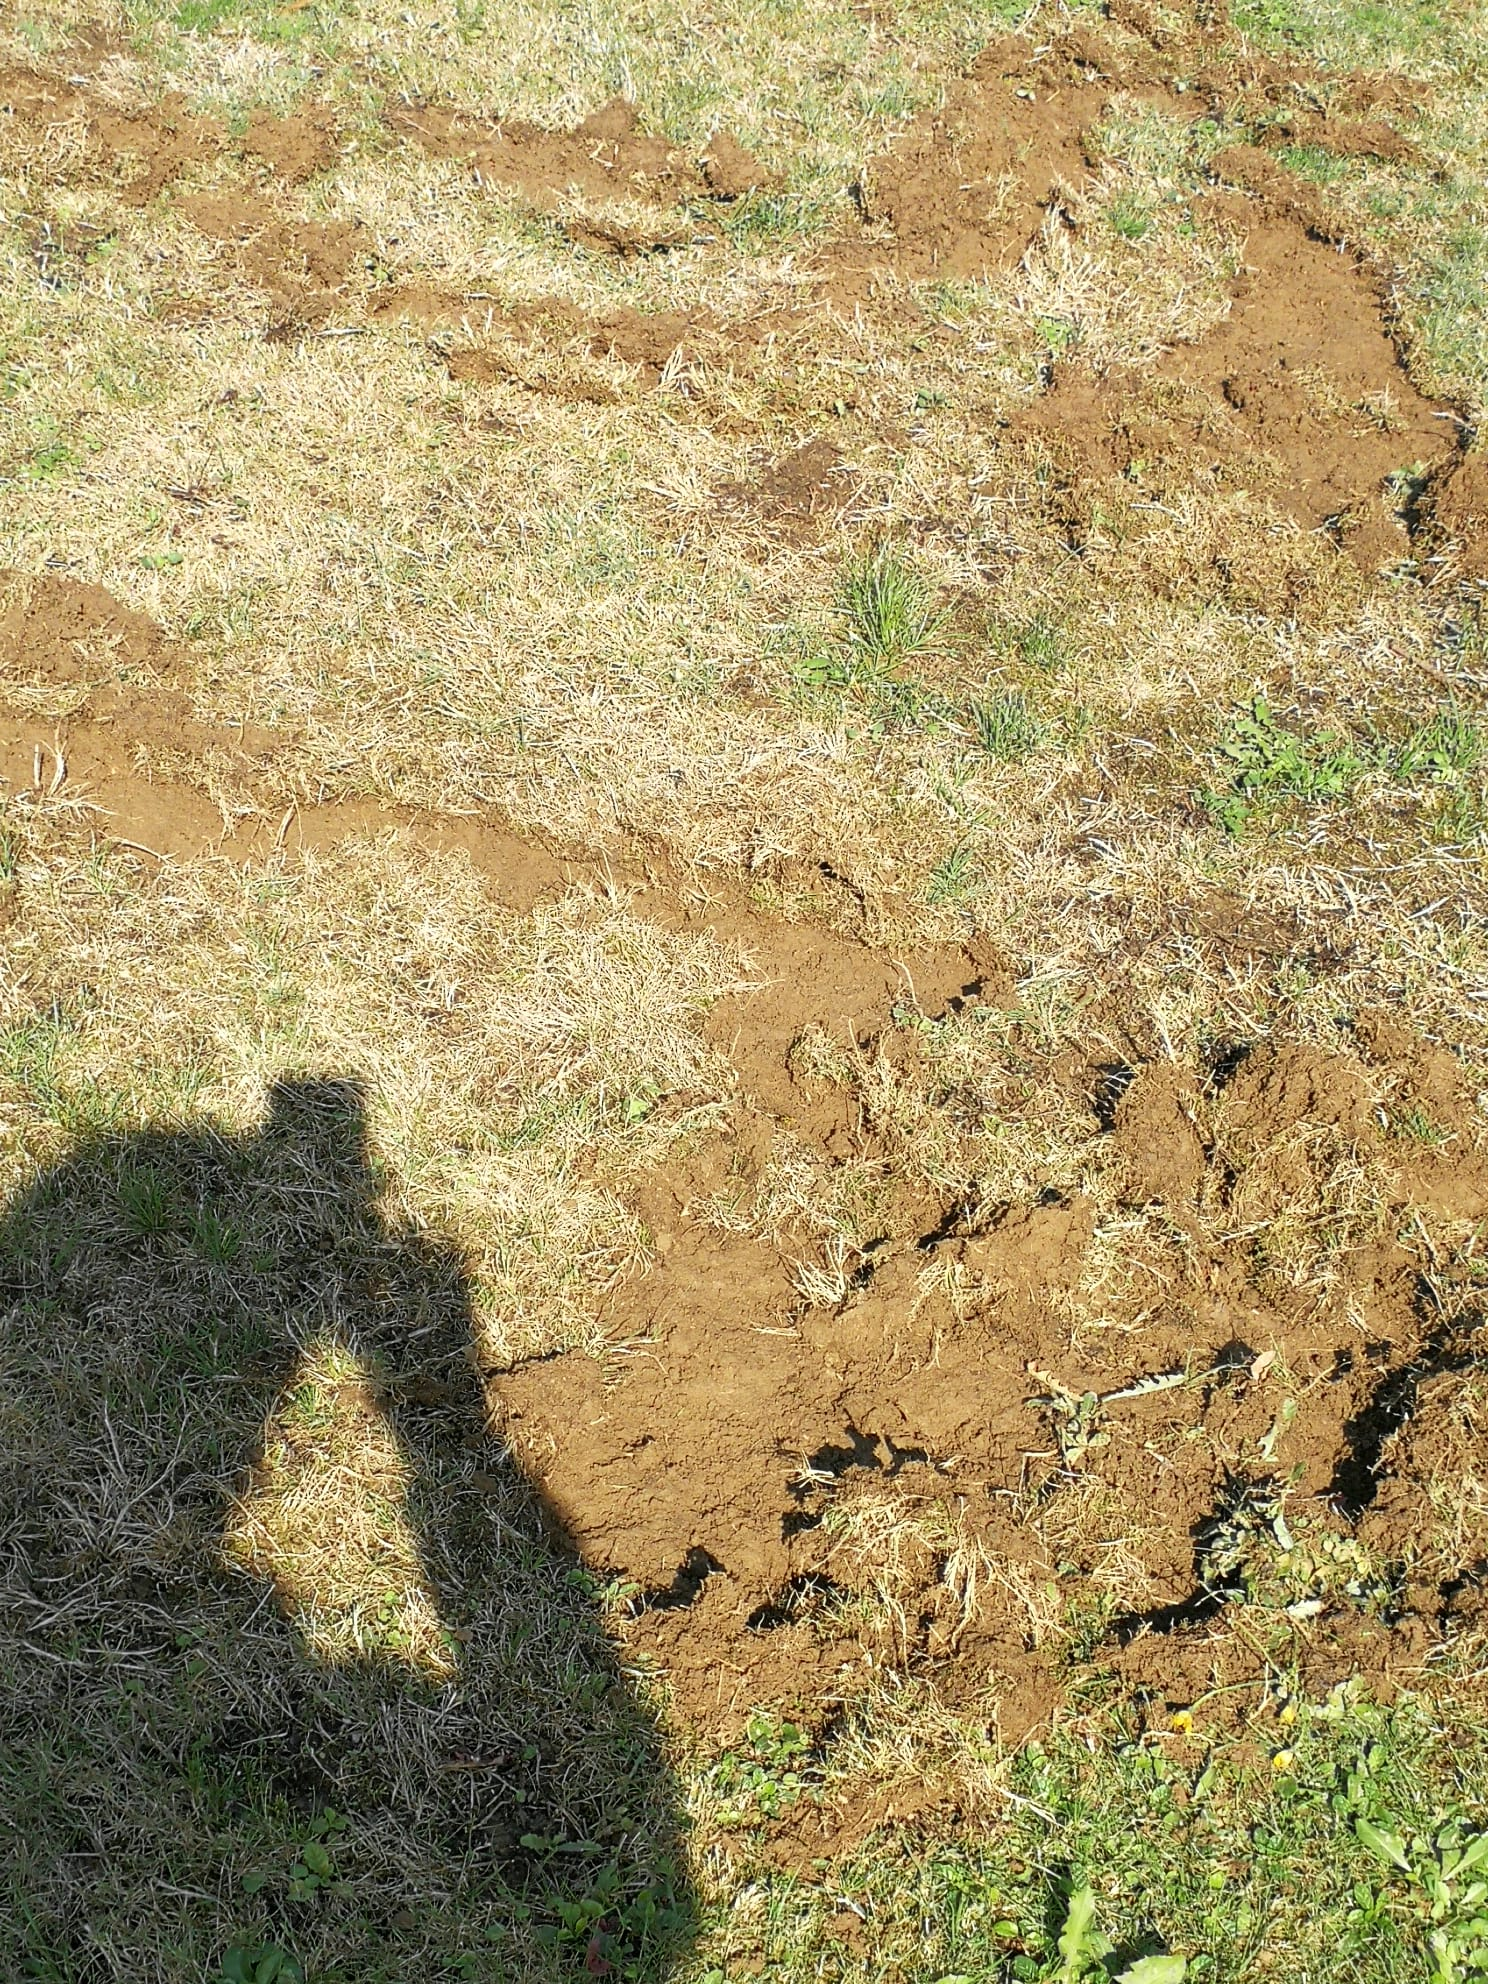
\includegraphics[angle=90,width=\textwidth]{images/Racoon_garden_ruin_0.jpeg}
    \caption[Verwüsteter Garten]{Ein durch Waschbären verwüsteter Garten}
    \label{fig:Garten}
\end{figure}


\section{Zielsetzung}

Das Ziel der Arbeit ist es, ein Abschrecksystem zur Fernhaltung von Mardern und Waschbären von privaten Grundstücken zu entwickeln. Im System soll eine Kombination von üblichen Abschreckungsmitteln aus den Baumarkt, einschließlich eines kleinen Wasserwerfers eingebaut sein. Darüber hinaus soll es aus Gründen der einfachen Anwendbarkeit portable an jeglichen Stellen im heimischen Garten aufgebaut werden können. Um zu verhindern das das Abschrecksystem unschuldige Passenten unter Beschuss nimmt, muss das System zwischen Mensch und Tier unterscheiden können.

\section{Aufgabenstellung}

Um die geplanten Ziele zu erfüllen, sind drei Kernelemente herauszuarbeiten. Zum einen soll das System portable sein, das heißt es muss sich selbst mit Energie für einen längeren Zeitraum versorgen können. Dazu bedeutet es die Wasserwerfer-Komponente auch mit Energie und Wasser versorgen zu können. Deshalb muss zusätzlich zur Energieversorgung ein Konzept für die Wasserversorgung erarbeitet werden. Zum anderen darf es nicht zu sperrig werden, damit es problemlos überall im Garten platziert werden kann. Hier könnten Abstriche hingenommen werden, falls die restlichen Funktionalitäten wie die eigenständige Energieversorgung oder den Einbau eines "Wasserwerfers" gewährleistet werden kann.
\\
Der Haupteil der Arbeit liegt aber bei der Unterscheidung zwischen einem tierischen Eindringling und einem menschlichen Passanten. Hierfür bieten sich Bilderkennungssoftware an die einen Eindringling von einem Passanten unterscheiden können.\\
Basierend darauf soll ein Prototype entwickelt werden, der möglichst all die Voraussetzungen erfüllen kann. Dieser Prototyp soll dazu dienen die Funktionsweise des Abschrecksystems im konzeptionellen Anwendungsfall zu demonstrieren und zu veranschaulichen.
